\chapter{Introduction}
\section{Delaunay Triangulation}
% \textcolor{blue}{(Start from Voronoi Diagram?)}

Suppose we have a finite set of points $S$ in the Euclidean plane. A triangulation of $S$ is called a Delaunay triangulation if the circumscribed circles of every triangle is empty. Notice that we say a circle is empty if there is no point in the point set in its interior. We can also define the Delaunay triangulation in the term of edges. That is, an edge $xy$ is in the Delaunay triangulation if and only if there is a empty circle passing through points $x$ and $y$. The Delaunay triangulation and Voronoi diagram are dual to each other.
Figure~\ref{fig:DTEx} gives an example for the Delaunay triangulation. 



\begin{figure}[ht]
\begin{subfigure}{0.31\textwidth}
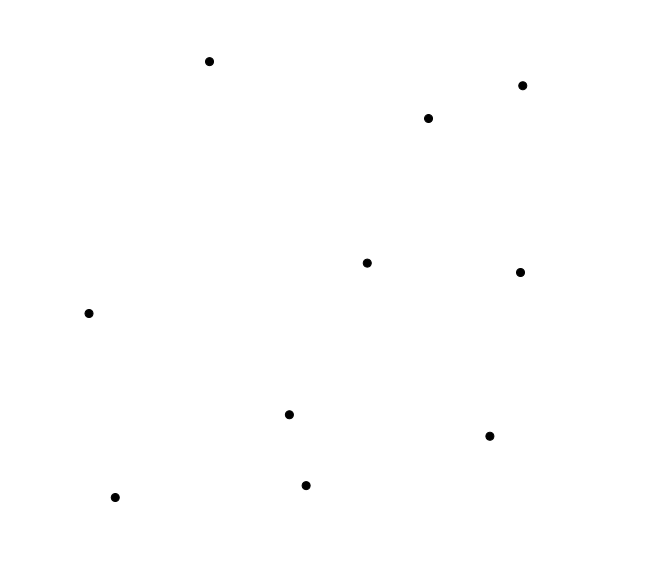
\includegraphics[width=\linewidth]{Figures/DTEx_a.png}
\caption{} \label{fig:DTEx_a}
\end{subfigure}
\hspace*{\fill} % separation between the subfigures
\begin{subfigure}{0.31\textwidth}
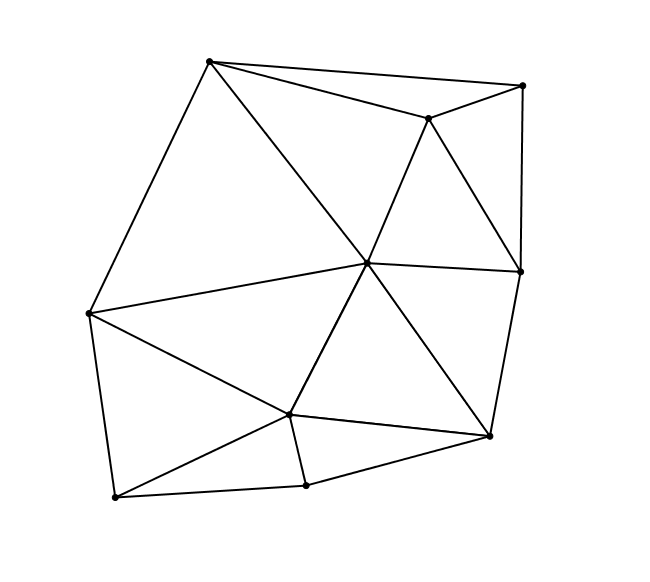
\includegraphics[width=\linewidth]{Figures/DTEx_b.png}
\caption{} \label{fig:DTEx_b}
\end{subfigure}
\hspace*{\fill} % separation between the subfigures
\begin{subfigure}{0.31\textwidth}
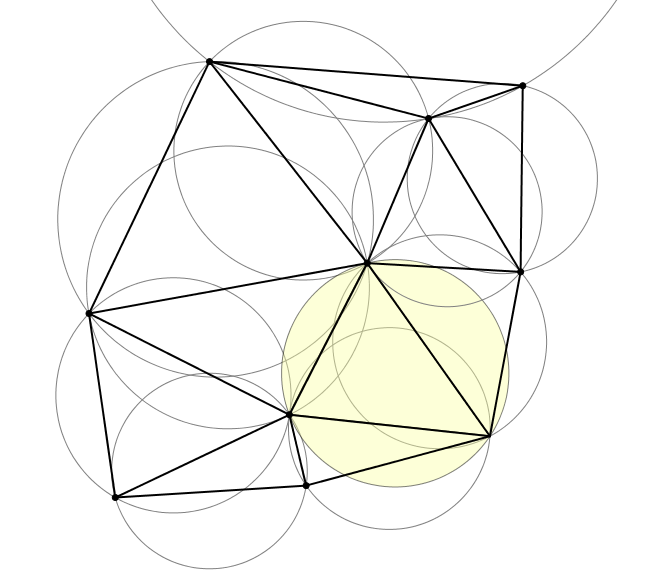
\includegraphics[width=\linewidth]{Figures/DTEx_c.png}
\caption{} \label{fig:DTEx_c}
\end{subfigure}
\caption[An example for the Delaney triangulation.]{An example for the Delaney triangulation.  In \ref{fig:DTEx_a}, a finite set of points is given. Its Delaunay triangulation is illustrated in \ref{fig:DTEx_b}. \ref{fig:DTEx_c} labels the circumscribed circle of every triangle in blue. Adapted from Wikipedia\cite{wiki:DT}.} \label{fig:DTEx}
\end{figure}



\section{ Stretch Factor}
The stretch factor $\rho$ of the Delaunay triangulation $D$ is the maximum ratio, among all points $p$ and $q$ in $S$, of the shortest path distance from p to q in $D$ over the Euclidean distance $\|pq\|$. The formula is provided as the following.
\[\rho(D) = \max_{\forall{p, q\in S}}\frac{{\min{|P(p, q)|}}}{||pq||}.\]

The concept of stretch factor have some other names such as dilation, spanning ratio or distortion.
In this thesis, we investigate the tight bound on the stretch factor of the Delaunay triangulation.  





\section{Arcgons}
We define a \textbf{disk} $d$ is the region in a Euclidean plane bounded by a circle $c$. 
Then,  a graph $f$ is  a \textbf{face} if its edges are the boundary of a convex subset of a disk $d$, and its vertices are on the boundary of $d$. 
Thus, the edges of a face is either circular arcs or straight lines. We say the circle $c$ is the \textbf{base circle} of the face $f$.

A \textbf{circles segment} is a region  bounded by an arc and the chord connecting the endpoints of the arc. Then, a \textbf{face on circle segment} is a graph whose edges are the boundary of a circle segment, and vertices are the two endpoints of the arc.


An \textbf{arcgon} is a planar graph defined as a finite sequence of distinct faces $F = \{f_1, f_2, \dots, f_n\}$ that meets the following conditions.
\begin{enumerate}

    \item The two ends $f_1$ and $f_n$ are faces on circle segment with a special vertex on the circular arc edge called  the \textbf{terminal point}. Denote the terminal points on $f_1$ and $f_n$  as $p$ and $q$ respectively. 
    \item For every two consecutive faces $f_i$ and $f_{i+1}$, $1\le i\le n-1$, none of the circular arcs of $f_i$ and $f_{i+1}$ intersects, and exactly one straight line edge of $f_i$ is also a straight line edge of $f_{i+1}$. Those interior straight line edges are called as \textbf{diagonals}.
    \item The union of regions bounded by all faces in $F$ has a boundary constructed by curricular arcs. That is, the outsider boundary contains only circular arc edges. 
    \item (Local Delaunay) Vertices of every  face $f_i$, $1\le i\le n-1$, lie either on or outside the base circles of neighboring faces $f_{i-1}$ and $f_{i+1}$.
    \item ($pq$-Delaunay) $p$ and $q$ are either on or outside all basic circles of faces in $F$.
    \item (Realizability) All diagonals intersect the segment $\overline{pq}$ at some points except their ends.
\end{enumerate}

Define the \textbf{stretch factor} of an arcgon $A$ as the ratio of the shortest path distance between the terminal points $p$ and $q$ over the their Euclidean distance $||pq||$. 


The definition of arcgons is well defined so that studying the tight bound on the stretch factor of arcgons is equivalent to studying on the the stretch factor of Delaney triangulation. Given a Delaunay triangulation of a point set, and suppose its stretch factor is $\rho$. Since the stretch factor of Delaney triangulation is defined as the max ratio over all pair of points, we can always choose a pair of some points $p$ and $q$ such that the ratio of their shortest path over their Euclidean distance is $\rho$ and none pairs of points has a ratio greater than that. Then, consider all triangles passed by $\overline{pq}$. Take their circumcircles as our base circle of faces. And construct an arcgon based on those faces. Then, the stretch factor of the arcgon is not less than $\rho$. That is, if we prove the stretch factor of an arcgon is at most $\kappa$, we can say that the stretch factor of a Delaney triangulation must be at most $\kappa$. 


The argument above shows an upper bound for the stretch factor of arcgons is an upper bound for that of Delaunay triangulation. On the other hand, since we can always convert an arcgons to a Delaunay triangulation, it is clear that a lower bound for the stretch factor of arcgons will be a lower bound for that of Delaunay triangulation. Therefore, since the tight bound for the stretch factor of arcgons is equivalent to that of Delaunay triangulation, we will focus on the arcgons instead in this thesis.




We say an edge $e$ of an arcgon is \textbf{critical} if there is a shortest path between $p$ and $q$ passing through $e$. If all edges in an arcgon is critical, the arcgon is a \textbf{critical arcgon}. 



An arcgon is \textbf{symmetric} if there is a line $l$ in the plane perpendicular to $pq$ such that the reflection of the arcgon with respective to $l$ is the same as the arcgon. Then, we say a \textbf{symmetric critical arcgon} is an arcgon if it is symmetric and critical.









\section{Applications}
The stretch factor of the Delaunay triangulation has wide applications.
\subsection{Network Design}
In 1989, Chew\cite{chew} mentioned that network design would an application.  Consider servers as vertices and channels between servers as edges. Then, using Delaunay triangulation to construct a network may close to give the optimal solutions. First, the network we develop in Delaunay triangulation is planar. Thus, only the linear number of edges are needed. This property could significantly reduce the complexity of problems relative to network. Also, the worst transmission distance between two sites are bounded. According to  the lower bound of the stretch factor shown in \cite{xia}, the shortest path distance between two servers would not be greater than $1.998$ times the physical distance.

In 2003, Li, Calinescu, Wan and Wang\cite{ad} the application of Delaunay triangulation in wireless computing, in particular, ad hoc wireless networks. An ad hoc  wireless network is a type of computer-to-computer connection. Users do not need to connect with Wi-Fi to communicate with each other. That is, a computer can build up a wireless connection directly to another computer. If the built-in network topology is the Delaunay triangulation, some localized routing protocols will guarantee the delivery of the packets. Then, the total distance traveled by the packet over the physical distance is our stretch factor. Therefore, improving the bound on the stretch factor of the Delaunay triangulation will directly prove the performance of wireless computing. 





\subsection{Motion Planning Problem}
A motion planning problem is to find the best path moving from a start configuration  $S$ to a goal configuration $G$, while avoiding collision with known obstacles. Chew \cite{chew} discussed the connection between this problem and Delaunay triangulation, in particular,  the constrained Delaunay triangulation. A constrained Delaunay triangulation is a generalization of the Delaunay triangulation that forces certain required segments into the triangulation. Figure~\ref{fig:CDT} gives a comparison between an ordinary Delaunay triangulation and a constrained Delaunay triangulation. 



\begin{figure}[ht]
\centering
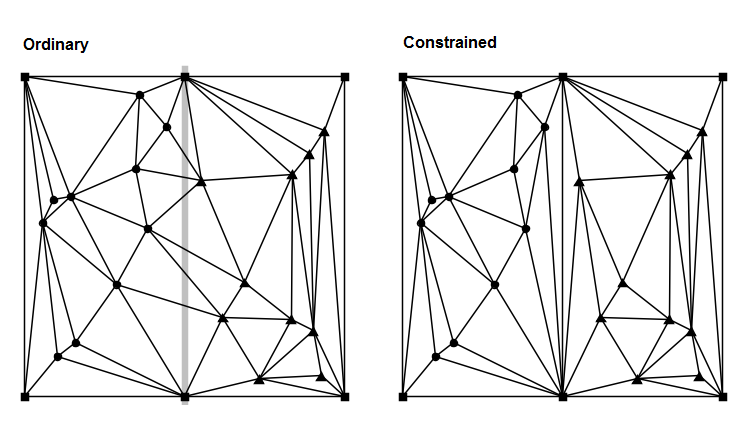
\includegraphics[width=80mm]{Figures/CDT.png}
\caption[A Delaunay triangulation and a constrained Delaunay triangulation.]{A Delaunay triangulation and a constrained Delaunay triangulation. The  ordinary one on the left hand side is a Delaunay triangulation. Suppose there is an obstacle in the middle of the graph as shown in gray. Our triangulation is constrained, and there must be a edge in the place of the obstacle. Reprinted form \cite{github}.} 
\label{fig:CDT}
\end{figure}

Constrained Delaunay triangulation is largely applied in the field of topographic surveying. Consider there is a river crosses some edges in the triangulation based on a city. That is, the original designed paths do not accurately describe the path of the river. Then, by adding the river as a breakline in the triangulation, the graph could better model the possible paths between vertices. Anderson, Karumanchi and Iagnemma explained the application of constrained Delaunay triangulation in semi-autonomous vehicles. Figure~\ref{fig:auto} shows the model of path planning using constrained Delaunay triangulation.

\begin{figure}[ht]
\centering
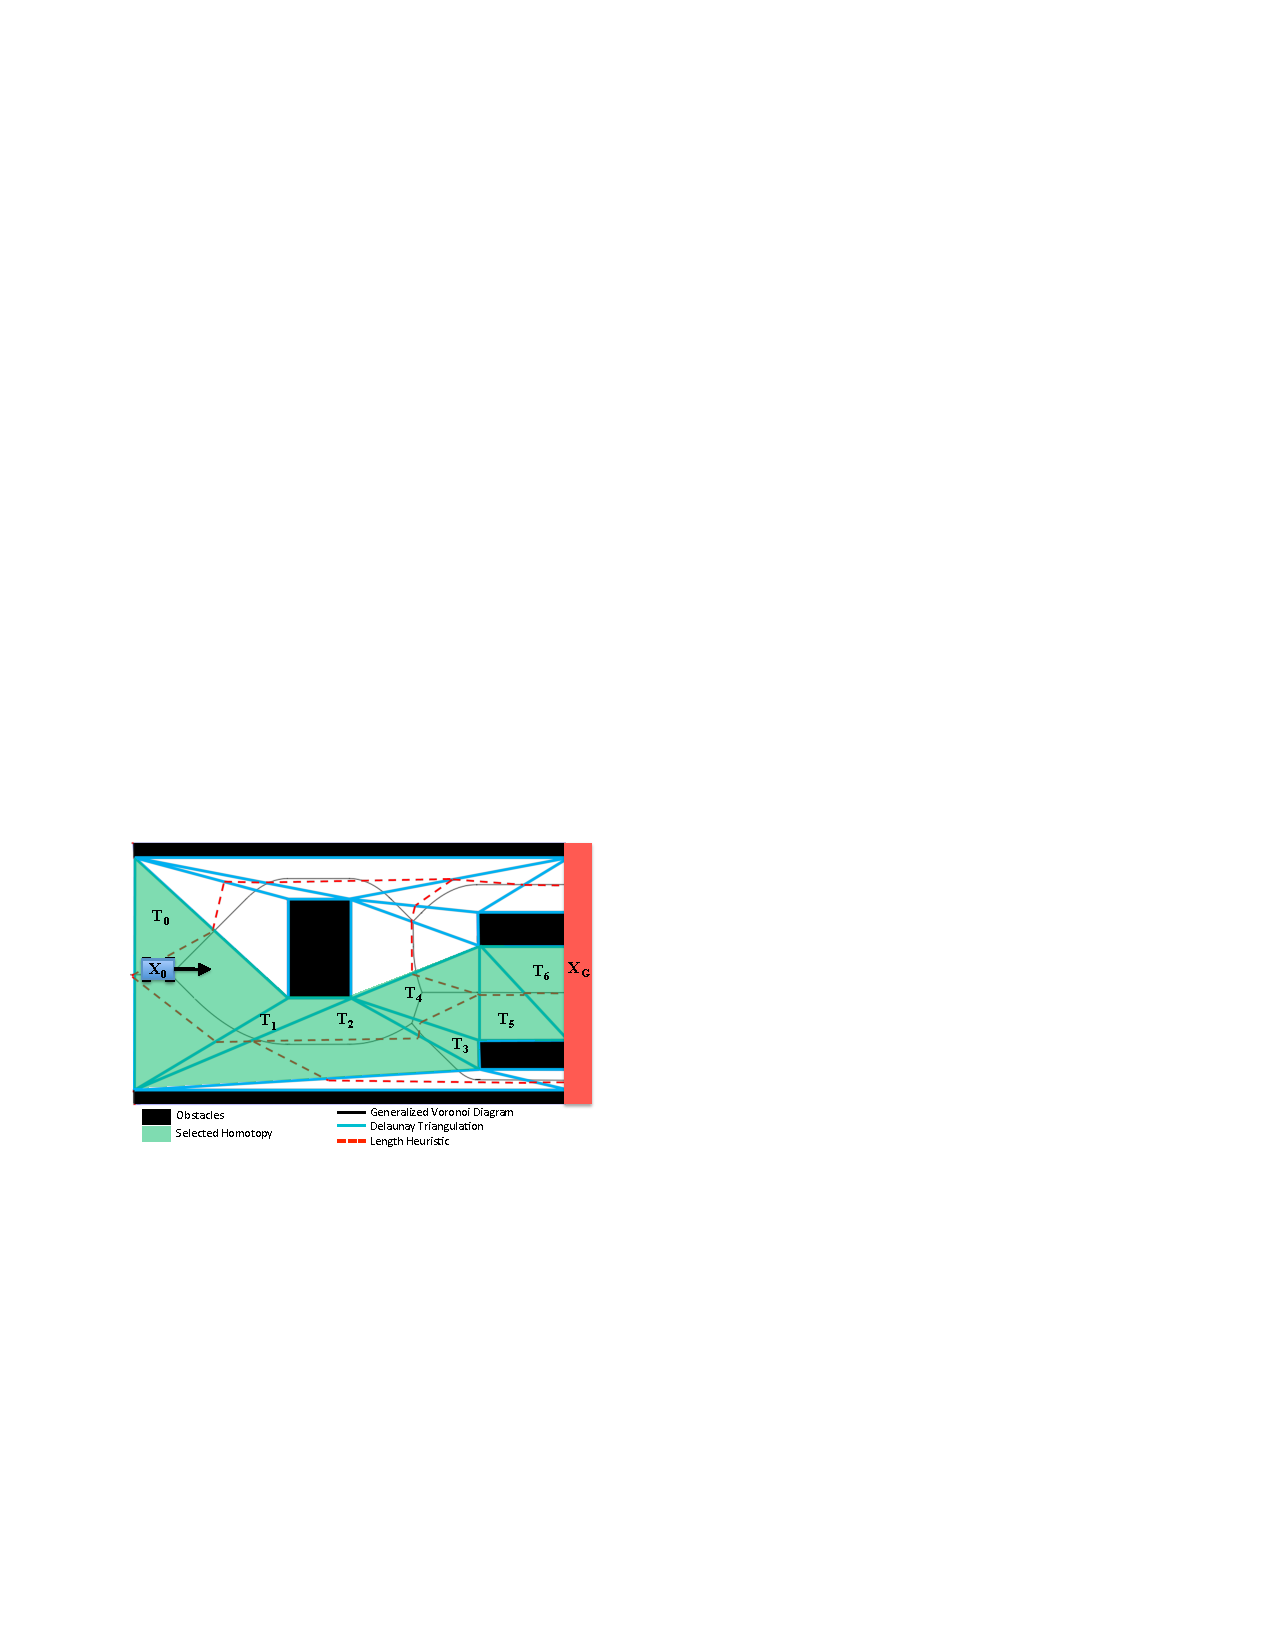
\includegraphics[width=100mm]{Figures/auto.pdf}
\caption[Constrained Delaunay triangulation in path planning in Automated driving]{Constrained Delaunay triangulation in path planning in Automated driving. Reprinted form \cite{auto}.} 
\label{fig:auto}
\end{figure}




\section{Organization of the Thesis}
In this thesis, we focus on the stretch factor of a special case in Delaunay triangulation, the symmetric critical arcgon. In section 3, we derive formula for our basic case, the stretch factor of symmetric critical arcgons with three circles. Section 4 gives a general formula. Then, we attempt to improve both the lower and upper bounds. section 5 illustrates how we show the existence of some worse stretch factor with the general formula in section 3. And section 6 provides a complete proof showing that an upper bound of stretch factors for all symmetric critical arcgons with  three circles is $1.6$. 